% 103-89(103쪽) — 밑면의 가로의 길이가 1 m 인 직육면체 모양의 상자(보이지 않는 모서리는 점선).
% 스캔 화질이 낮아 TikZ 로 다시 그림. 라벨은 원문 그대로 밑면 앞 모서리의 1 m 만 두고
% 부피·높이(답)는 그림에 나타내지 않는다.
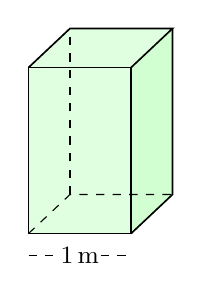
\begin{tikzpicture}[scale=0.62, line width=0.6pt]
  \coordinate (FBL) at (0,0); \coordinate (FBR) at (2.1,0);
  \coordinate (FTR) at (2.1,3.4); \coordinate (FTL) at (0,3.4);
  \coordinate (BBL) at (0.85,0.8); \coordinate (BBR) at (2.95,0.8);
  \coordinate (BTR) at (2.95,4.2); \coordinate (BTL) at (0.85,4.2);
  \fill[green!12] (FBL) -- (FBR) -- (FTR) -- (FTL) -- cycle;
  \fill[green!12] (FTL) -- (BTL) -- (BTR) -- (FTR) -- cycle;
  \fill[green!18] (FBR) -- (BBR) -- (BTR) -- (FTR) -- cycle;
  \draw (FBL) -- (FBR) -- (FTR) -- (FTL) -- cycle;
  \draw (FTL) -- (BTL) -- (BTR) -- (FTR);
  \draw (FBR) -- (BBR) -- (BTR);
  \draw[dashed, line width=0.4pt] (FBL) -- (BBL) -- (BBR);
  \draw[dashed, line width=0.4pt] (BBL) -- (BTL);
  \draw[dashed, line width=0.4pt] (0,-0.45) -- (0.62,-0.45);
  \draw[dashed, line width=0.4pt] (1.48,-0.45) -- (2.1,-0.45);
  \node[font=\small] at (1.05,-0.45) {$1\,\mathrm{m}$};
\end{tikzpicture}
